\documentclass[12pt]{report}
%	options include 12pt or 11pt or 10pt
%	classes include article, report, book, letter, thesis
\usepackage{graphicx}

\title{Wings Of War}
\author{Aversa - Di Cicco - Nenci}

\begin{document}
\maketitle
\tableofcontents
\chapter{Introduction}

\section{AI in games}

\section{AI to move characters}
One of the most fundamental requirements of AI is to move characters around in the game sensibly. Even the earliest AI-controlled characters (the ghosts in Pac-Man, for example, or the opposing bat in some Pong variants) had movement algorithms that weren’t far removed from the games on the shelf today. Movement forms the lowest level of AI techniques. Many games, including some with quite decent-looking AI, rely solely on movement algorithms and don’t have any more advanced decision making. At the other extreme, some games don’t need moving characters at all. Resource management games and turn-based games often don’t need movement algorithms; once a decision is made where to move, the character can simply be placed there.

All movement algorithms have this same basic form. They take geometric data about their
own state and the state of the world, and they come up with a geometric output representing the movement they would like to make.
Some movement algorithms require very little input: the position of the character and the
position of an enemy to chase, for example. Others require a lot of interaction with the game
state and the level geometry. A movement algorithm that avoids bumping into walls, for example, needs to have access to the geometry of the wall to check for potential collisions.

\section{Turn based games}
Decision making is the ability of a character to decide what to do.
decision making is typically a small part of the effort needed to build great game
AI. Most games use very simple decision making systems: state machines and decision trees.
Rule-based systems are rarer, but important.
The character processes a set of information that it uses to generate an action that it wants to
carry out. The input to the decision making system is the knowledge that a character possesses,
and the output is an action request. The knowledge can be further broken down into external
and internal knowledge. External knowledge is the information that a character knows about the
game environment around it: the position of other characters, the layout of the level, whether a
switch has been thrown, the direction that a noise is coming from, and so on. Internal knowledge
is information about the character’s internal state or thought processes: its health, its ultimate
goals, what it was doing a couple of seconds ago, and so on.
Typically, the same external knowledge can drive any of the algorithms in this chapter, whereas
the algorithms themselves control what kinds of internal knowledge can be used (although they
don’t constrain what that knowledge represents, in game terms)
\section{Research based approaches}
Decision trees are fast, easily implemented, and simple to understand. They are the simplest
decision making technique that we’ll look at, although extensions to the basic algorithm can make
them quite sophisticated. They are used extensively to control characters and for other in-game
decision making, such as animation control.
They have the advantage of being very modular and easy to create.
Given a set of knowledge, we need to generate a corresponding action from a set of possible
actions.
The mapping between input and output may be quite complex. The same action will be used
for many different sets of input, but any small change in one input value might make the difference
between an action being sensible and an action appearing stupid.
We need a method that can easily group lots of inputs together under one action, while
allowing the input values that are significant to control the output.




\chapter{Wings of War}

\section{The board game}

Wings of War is a game series which merges card and board game mechanics to recreate aerial combat.

Airplanes are represented by a single card which is used as a playing piece on any open surface; the players choose and \textbf{play simultaneously} movement cards to decide the actions of the airplane they control. Different planes use different decks of movement cards to represent their different maneuver capabilities, and different deck of "Fire" card are used to take into account their fighting effectiveness and to keep track of damage.

Each Wings of War set is a complete game for 2 to 4 players which may be combined with additional sets, or with other copies of the same set, to play larger games.

\begin{figure}
  \centering
      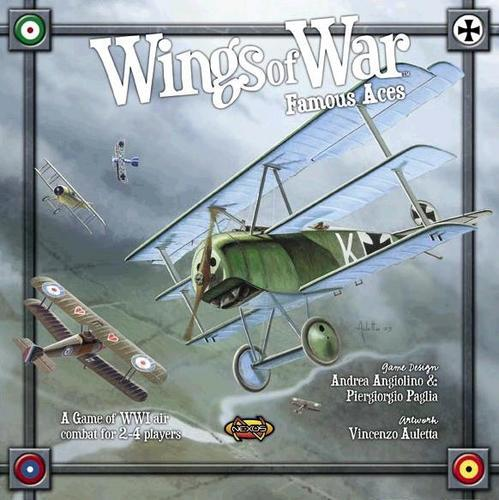
\includegraphics[width=0.5\textwidth]{images/wow.jpg}
  \caption{Wings Of War box}
\end{figure}

\section{Basic Rules}
\subsection{Preparation}
Each player chooses an equal number of airplane cards then he takes a gameboard for each plane and puts on it, in the proper place, a set of “Maneuver” cards, matching the blue letter on the airplane card.
The game can be played with more than one plane per player:maneuver planning, firing and damage account are made separately for each airplane. It also possible to play with more than two players, divided into teams.
\subsection{Game turn}
Each turn has a planning phase and three movement \& fire phases.
\subsection{Planning}
 At the start of the turn, each player chooses three cards fromeach of his planes’ maneuver decks. These cards are the three maneuvers that each plane will perform during that turn.
Certain maneuver cards need to be played after (or before) some specific cards.
\subsection{Movement}
When all the players have planned their moves, they reveal the first of their Maneuver cards for the turn (then the second and the third, in the same order of choice).
The planes are then moved using the right rigid cardboard guides.
\subsection{Firing}
After all planes have moved using their maneuver cards the players have to check if an airplane can fire at an opponent’s airplane using the rigid ruler. If the check is positive the airplane can fire at the opponent. It is possible that two planes can fire at each other. 
If the target airplane is reached by the first half of the ruler, it takes two cards of damage. If it is more distant and it is reached by the second half of the ruler, it takes only one card of damage. Fighter airplanes can fire at a single target each phase. It is forbidden to fire through another plane, enemy or friendly.
\subsection{Damage}
When an airplane is fired at, the owner of that plane takes the damage cards and secretly looks at them and adding at the past damages. When the total reaches or excedes the life points on the airplane card, the airplane is shot down and eliminated.
Only if the player draws a card with the cross symbol must he reveal it and the airplane that fired at him has jammed his guns and cannot fire after each of the next three maneuvers.
\textbf{All damage is resolved simultaneously} after all airplanes that can fire have fired. Therefore, a plane that is shot down may still fire the same phase in which it is shot down.
\subsection{Rest of the turn}
Each turn is composed of three game phases. After all airplanes that can fire have resolved their firing, the first game phase is ended. Everybody reveals the second maneuver card for the  turn. Move and resolve firing. Then reveal the third card, move  and resolve firing. Then the turn is finished and the planning  of the next one can begin.
\subsection{Overlapping}
If two airplane cards overlap, neither of the two airplanes can fire at each other until they move and don’t overlap any more. They can, however, still fire at other planes.Other planes can shoot at the overlapping planes using the normal rules.
\subsection{Exit from the gaming surface}
An airplane that goes out of the playing area with its central dot is out of the game.
\subsection{Victory}
The last player having one or more planes on the playing area after all the enemy ones have been eliminated or exited wins the match.

\section{Our game}
\label{modify this name} 
Our customization to game rules were made to simplify the game flow.

In a nutshell:
\begin{itemize}
    \item Two players (Ai vs Human)
    \item Reduced set of maneuver cards 
    \item Every shot always hits the target
    \item Exiting from the \textit{world} is a sudden death (and a game over)           
\end{itemize}

\subsection{Cards}
In the planning phase each player had to choose \textbf{three} from the available cards.

Available cards are:
\begin{itemize}
    \item Long/short forward thrust
    \item Long/short right turn
    \item Long/short left turn
\end{itemize}

\chapter{Heuristics}
Fatti
\chapter{The Brain}
Città
\chapter{Results}
Cani
\end{document} 